Un componente importante en las redes neuronales para el lenguaje es el uso de una capa de embedding.
Se trata de una asignación de símbolos discretos a vectores continuos.
Cuando se realiza el embedding de palabras, estas pasan de ser símbolos distintos y aislados a objetos matemáticos en los que se puede operar.
La distancia entre vectores puede equipararse a la distancia entre palabras.
Esto facilita generalizar el comportamiento de una palabra a otra.

\section{Hipótesis Distribucional y Matrices Palabra Contexto}
La \textbf{hipótesis distribucional} \cite{harris1954} establece que las palabras que ocurren en los mismos \textbf{contextos} tienden a tener significados similares.
O, en otras palabras, "una palabra se caracteriza por las compañías que mantiene".
Las \textbf{representaciones distribucionales} representan las palabras mediante \textbf{vectores de alta dimensionalidad} basados en los contextos en los que ocurren.

Los vectores distribucionales se construyen a partir de matrices de palabras-contexto $M$.
Cada celda $(i,j)$ es un valor de asociación basado en la co-ocurrencia entre una \textbf{palabra objetivo} $w_i$ y un \textbf{contexto} $c_j$, calculado a partir de un corpus de documentos.
Los contextos se definen comúnmente como ventanas de palabras que rodean a $w_i$.
La longitud de la ventana $k$ es un parámetro que va desde 1 hasta 8 palabras en ambos lados de $w_i$.
Si el vocabulario de las palabras objetivo y las palabras de contexto es el mismo, $M$ tiene una dimensionalidad de $|\mathcal{V}| \times |\mathcal{V}|$.
Mientras que las ventanas más cortas capturan información sintáctica (por ejemplo, POS), las ventanas más largas capturan más probabilidades de similitud temática \cite{goldberg2016primer, JurafskyBook}.

Ejemplo: Vectores de Distribución con ventanas contextuales de tamaño 1

\begin{figure}[htb]
\centering
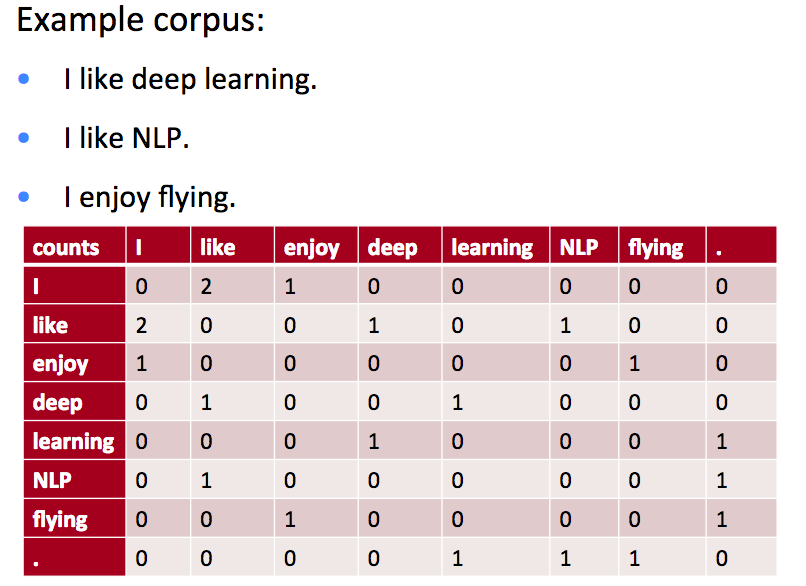
\includegraphics[scale=0.3]{pics/distributionalSocher.png}
\caption{Ejemplo tomado de: \url{http://cs224d.stanford.edu/lectures/CS224d-Lecture2.pdf}}
\end{figure}



Las asociaciones entre palabras y contextos se pueden calcular utilizando diferentes enfoques:
\begin{enumerate}
    \item Recuento de co-ocurrencias.
    \item Información mutua puntual positiva (PPMI, por sus siglas en inglés).
    \item Valores de significancia de una prueba t emparejada.
\end{enumerate}
Según \cite{JurafskyBook}, el más común de estos enfoques es PPMI.
Los métodos de distribución también se conocen como métodos basados en conteo.

\section{PPMI}
PPMI calcula el logaritmo de la probabilidad de que los pares palabra-contexto ocurran juntos en comparación con la probabilidad de que sean independientes.

\begin{equation}
 \operatorname{PMI}(w, c)= \log_2 \left( \frac{P(w,c)}{P(w)P(c)} \right) = \log_{2} \left ( \frac{\operatorname{count}(w,c)\times |D|}{\operatorname{count}(w)\times \operatorname{count}(c)} \right ) 
\end{equation}


Los valores de PMI negativos sugieren que la pareja ocurre menos a menudo de lo esperado por azar.
Estas estimaciones no son confiables a menos que los conteos se calculen a partir de corpus muy grandes \cite{JurafskyBook}.
PPMI corrige este problema reemplazando los valores negativos por cero.

\begin{equation}
 \operatorname{PPMI}(w, c)= \operatorname{max}(0,\operatorname{PMI}(w, c))
\end{equation}



Los vectores distribuidos o word embeddings son vectores continuos de palabras de baja dimensionalidad que se entrenan a partir de corpus de documentos utilizando redes neuronales.
El tamaño de los vectores de distribución basados en recuento aumenta con el vocabulario, es decir, pueden tener una dimensionalidad muy alta.
Almacenar explícitamente la matriz de co-ocurrencia puede requerir mucha memoria.
Algunos modelos de clasificación no escalan bien con datos de alta dimensionalidad.
La comunidad de redes neuronales prefiere utilizar representaciones \textbf{distribuidas}\footnote{Idea: El significado de la palabra está "distribuido" en una combinación de dimensiones.} o \textbf{word embeddings}.
Los word embeddings son vectores densos de palabras de baja dimensionalidad que se entrenan a partir de corpus de documentos utilizando redes neuronales.
Las dimensiones no son directamente interpretables, es decir, representan características latentes de la palabra, "capturando esperanzadamente propiedades sintácticas y semánticas útiles" \cite{turian2010word}.
Se han convertido en un componente crucial de las arquitecturas de redes neuronales para el procesamiento del lenguaje natural.


Existen dos enfoques principales para obtener word embeddings:

\begin{enumerate}
 \item Capas de embedding: utilizando una capa de embedding en una arquitectura de red neuronal específica para una tarea, entrenada a partir de ejemplos etiquetados (por ejemplo, análisis de sentimientos).
\item Word embeddings pre-entrenados: creando una tarea predictiva auxiliar a partir de corpus no etiquetados (por ejemplo, predecir la siguiente palabra) en la que los word embeddings surgirán naturalmente a partir de la arquitectura de la red neuronal.
\end{enumerate}



Estos enfoques también se pueden combinar: se puede inicializar una capa de embedding de una red neuronal específica para una tarea con word embeddings pre-entrenados obtenidos mediante el segundo enfoque.
Los modelos más populares basados en el segundo enfoque son skip-gram \cite{Mikolov2013}, continuous bag-of-words \cite{Mikolov2013} y GloVe \cite{penningtonSM14}.
Los word embeddings han demostrado ser más poderosos que los enfoques distribucionales en muchas tareas de procesamiento del lenguaje natural \cite{baroni2014don}.
En \cite{amir2015SemEval}, se utilizaron como características en un modelo de regresión para determinar la asociación entre palabras de Twitter y sentimientos positivos.


\section{Word2Vec}
Word2Vec es un paquete de software que implementa dos arquitecturas de redes neuronales para entrenar word embeddings: Continuous Bag of Words (CBOW) y Skip-gram.
Implementa dos modelos de optimización: Muestreo Negativo (Negative Sampling) y Softmax Jerárquico (Hierarchical Softmax).
Estos modelos son redes neuronales poco profundas que se entrenan para predecir los contextos de las palabras.
Se puede encontrar un tutorial muy completo sobre los algoritmos detrás de Word2Vec en \url{https://arxiv.org/pdf/1411.2738.pdf}.

El modelo Skip-gram entrena una red neuronal con una capa oculta para predecir las palabras que rodean a una palabra central, dentro de una ventana de tamaño $k$ que se desplaza a lo largo del corpus de entrada.
La palabra central y las $k$ palabras circundantes corresponden a las capas de entrada y salida de la red.
Inicialmente, las palabras se representan mediante vectores one-hot: vectores del tamaño del vocabulario ($|V|$) con valores cero en todas las entradas excepto en el índice correspondiente a la palabra, que recibe un valor de 1.


La capa de salida combina los $k$ vectores one-hot de las palabras circundantes.
La capa oculta tiene una dimensionalidad $d$, que determina el tamaño de los embeddings (normalmente $d \ll |V|$).

\begin{figure}[h]
\centering
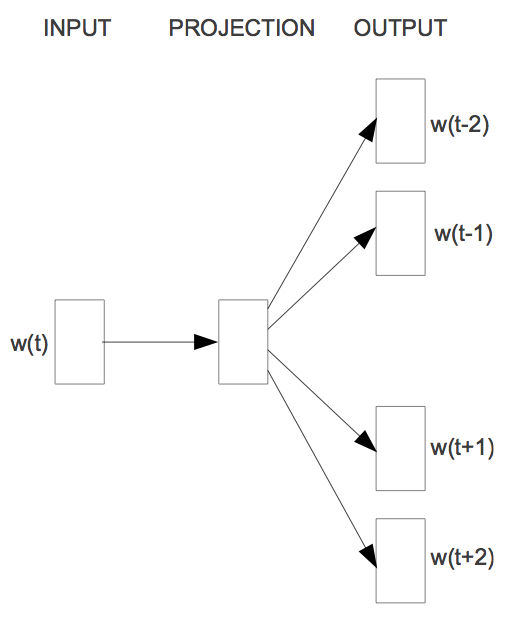
\includegraphics[scale=0.4]{pics/skip-gram.png}
\caption{Imagen tomada del artículo original}
\end{figure}

\begin{figure}[h]
\centering
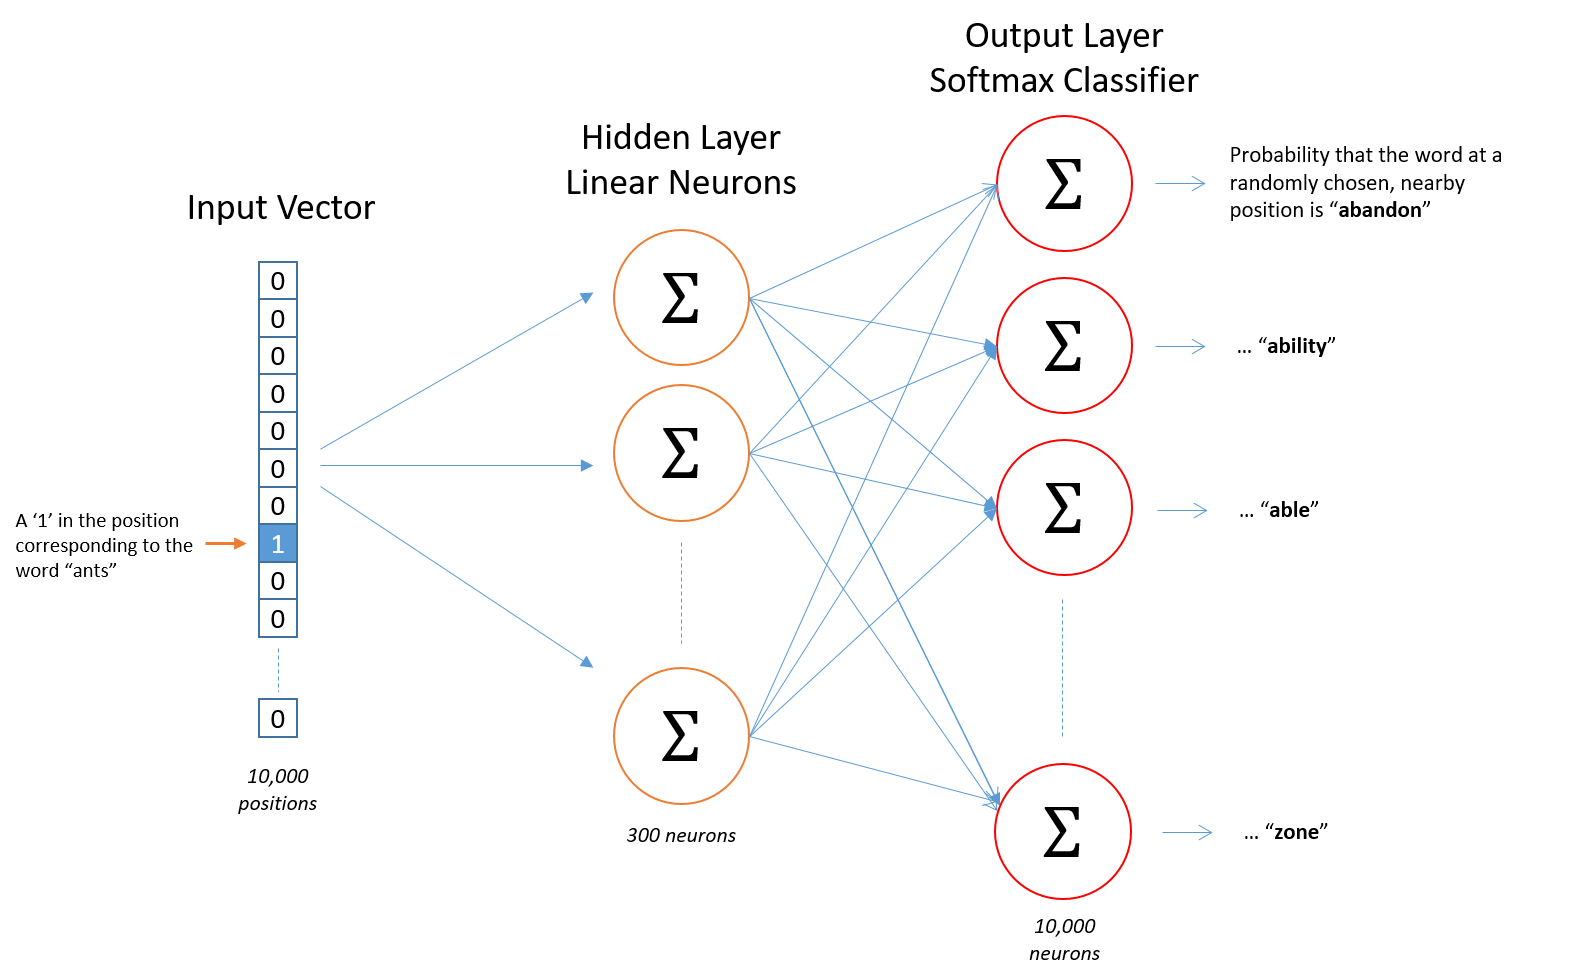
\includegraphics[scale=0.4]{pics/skip_gram_net_arch.png}
\caption{Imagen tomada de: \url{http://mccormickml.com/2016/04/19/word2vec-tutorial-the-skip-gram-model/}}
\end{figure}



El modelo Skip-gram utiliza un softmax jerárquico donde el vocabulario se representa como un árbol binario de Huffman.
Esto se basa en observaciones anteriores de que la frecuencia de las palabras funciona bien para obtener clases en modelos de lenguaje basados en redes neuronales.
Los árboles de Huffman asignan códigos binarios cortos a palabras frecuentes, lo que reduce aún más el número de unidades de salida que deben evaluarse.

Si dos palabras diferentes tienen contextos muy similares (es decir, qué palabras es probable que aparezcan a su alrededor), entonces nuestro modelo necesita generar resultados muy similares para estas dos palabras.
Y una forma de lograr que la red genere predicciones de contexto similares para estas dos palabras es si los vectores de palabras son similares.
Por lo tanto, si dos palabras tienen contextos similares, ¡nuestra red estará motivada a aprender vectores de palabras similares para estas dos palabras! ¡Ta-da!

¿Y qué significa que dos palabras tengan contextos similares? Creo que se podría esperar que sinónimos como "inteligente" y "astuto" tengan contextos muy similares.
O que palabras relacionadas, como "motor" y "transmisión", probablemente también tengan contextos similares.

\subsection{Parametrización del modelo Skip-gram}

Se nos proporciona un corpus de entrada formado por una secuencia de palabras $w_1, w_2, w_3, . . . , w_T$ y un tamaño de ventana $k$.

Denotamos las palabras objetivo o centrales con la letra $w$ y las palabras de contexto circundantes con la letra $c$.

La ventana de contexto $c_{1:k}$ de la palabra $w_t$ corresponde a las palabras $w_{t-k/2},\dots, w_{t-1}, w_{t+1}, \dots, w_{t+k/2}$ (asumiendo que $k$ es un número par).

El objetivo del modelo Skip-gram es maximizar la log-probabilidad promedio de las palabras de contexto dadas las palabras objetivo:

\begin{displaymath}
\frac{1}{T} \sum_{t=1}^T \sum_{c \in c_{1:k}} \log P(c|w_t)
\end{displaymath}

La probabilidad condicional de una palabra de contexto $c$ dada una palabra central $w$ se modela con una softmax ($C$ es el conjunto de todas las palabras de contexto, que generalmente es igual al vocabulario):

\begin{displaymath}
P(c|w) = \frac{e^{\vec{c}\cdot \vec{w}}}{\sum_{c'\in C} e^{\vec{c}'\cdot \vec{w}}}
\end{displaymath}

Los parámetros del modelo $\theta$ son $\vec{c}$ y $\vec{w}$ (representaciones vectoriales de los contextos y las palabras objetivo).

Sea $D$ el conjunto de pares palabra-contexto correctos (es decir, pares de palabras que se observan en el corpus).

El objetivo de optimización es maximizar la log-verosimilitud condicional de los contextos $c$ (lo cual es equivalente a minimizar la pérdida de entropía cruzada):

\begin{equation}
\begin{split}
\operatorname{arg} \max_{\vec{c}, \vec{w}} & \quad \sum_{(w,c) \in D}{\log P(c|w)} = \sum_{(w,c) \in D} ( \log e^{\vec{c}\cdot \vec{w}} - \log \sum_{c'\in C} e^{\vec{c}'\cdot \vec{w}} )
\end{split}
\end{equation}

Suposición: maximizar esta función resultará en buenos embeddings $\vec{w}$, es decir, palabras similares tendrán vectores similares.

El término $P(c|w)$ es computacionalmente costoso debido a la suma $\sum_{c'\in C} e^{\vec{c}'\cdot \vec{w}}$ sobre todos los contextos $c'$.

Solución: reemplazar la softmax por una softmax jerárquica (el vocabulario se representa con un árbol binario de Huffman).

Los árboles de Huffman asignan códigos binarios cortos a palabras frecuentes, lo que reduce el número de unidades de salida que deben evaluarse.

La hipótesis de distribución establece que las palabras en contextos similares tienen significados similares. El objetivo anterior claramente trata de aumentar la cantidad de buenos pares palabra-contexto y disminuirla para los malos. Int

uitivamente, esto significa que las palabras que comparten muchos contextos serán similares entre sí (también se observa que los contextos que comparten muchas palabras también serán similares entre sí). Sin embargo, esto es muy simplista.

Fuente: \url{https://arxiv.org/pdf/1402.3722.pdf}

El modelo Skip-gram y el Negative Sampling no son lo mismo.

\subsection{Skip-gram con Negative Sampling}

El Negative Sampling (NS) se presenta como un modelo más eficiente para calcular los embeddings del Skip-gram.
Sin embargo, optimiza una función objetivo diferente \cite{goldberg2014word2vec}.

El NS maximiza la probabilidad de que un par palabra-contexto $(w, c)$ provenga del conjunto de pares palabra-contexto correctos $D$ utilizando una función sigmoide:

\begin{displaymath}
P(D = 1| w,c_i) = \frac{1}{1+e^{-\vec{w} \cdot \vec{c_{i}}}}
\end{displaymath}

Suposición: las palabras de contexto $c_i$ son independientes entre sí:

\begin{displaymath}
P(D = 1| w,c_{1:k}) = \prod_{i=1}^{k}{P(D = 1| w,c_i)} = \prod_{i=1}^{k}{\frac{1}{1+e^{-\vec{w} \cdot \vec{c_{i}}}}} 
\end{displaymath}

Esto conduce a la siguiente función objetivo (log-verosimilitud):

\begin{equation}
\begin{split}
\operatorname{arg} \max_{\vec{c}, \vec{w}} & \quad \log P(D = 1| w,c_{1:k}) = \sum_{i=1}^{k}{\log \frac{1}{1+e^{-\vec{w} \cdot \vec{c_{i}}}}}
\end{split}
\end{equation}

Esta función objetivo tiene una solución trivial si establecemos $\vec{w}$, $\vec{c}$ de manera que $P(D=1|w,c)=1$ para cada par $(w,c)$ de $D$.
Esto se logra estableciendo $\vec{w}=\vec{c}$ y $\vec{w} \cdot \vec{c} = K$ para todos los $\vec{w}$, $\vec{c}$, donde $K$ es un número grande.
Necesitamos un mecanismo que evite que todos los vectores tengan el mismo valor, al no permitir algunas combinaciones $(w, c)$.
Una forma de hacerlo es presentarle al modelo algunos pares $(w, c)$ para los cuales $P(D=1|w, c)$ debe ser bajo, es decir, pares que no están en los datos.
Esto se logra muestreando ejemplos negativos de $\tilde{D}$.
Se muestrean $m$ palabras para cada par palabra-contexto $(w,c) \in D$.
Se agrega cada palabra muestreada $w_i$ junto con el contexto original $c$ como un ejemplo negativo en $\tilde{D}$.
$\tilde{D}$ es $m$ veces más grande que $D$.
El número de ejemplos negativos $m$ es un parámetro del algoritmo.

Función objetivo final:

\begin{equation}
\begin{split}
\operatorname{arg} \max_{\vec{c}, \vec{w}} & \quad \sum_{(w,c) \in D}{\log P(D = 1| w,c_{1:k})} + \sum_{(w,c) \in \tilde{D}} \log P(D = 0| w,c_{1:k})
\end{split}
\end{equation}

Las palabras negativas se muestrean a partir de una versión suavizada de las frecuencias del corpus:

\begin{displaymath}
\frac{\#(w)^{0.75}}{\sum_{w'}\#(w')^{0.75}}
\end{displaymath}

Esto otorga más peso relativo a las palabras menos frecuentes.

\subsection{Continuous Bag of Words: CBOW}

Similar al modelo Skip-gram, pero ahora se predice la palabra central a partir del contexto circundante.

\begin{figure}[h]
	\centering
	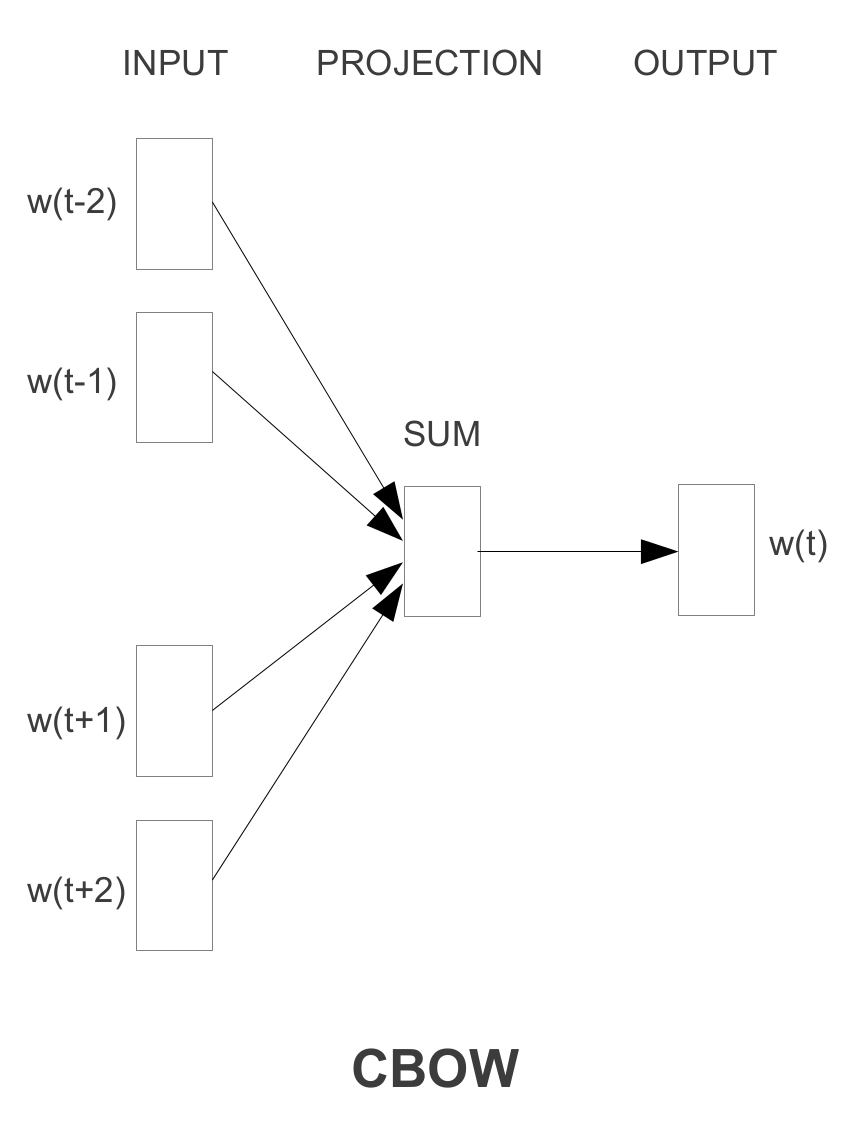
\includegraphics[scale=0.55]{pics/CBOW.png}
	\caption{Imagen tomada de: \url{http://mccormickml.com/2016/04/19/word2vec-tutorial-the-skip-gram-model/}}
\end{figure}

\subsection{GloVe}
GloVe (de global vectors) es otro método popular para entrenar word embeddings \cite{penningtonSM14}. Construye una matriz explícita palabra-contexto y entrena los vectores de palabra y contexto $\vec{w}$ y $\vec{c}$ intentando satisfacer la siguiente ecuación:

\begin{equation}
\vec{w} \cdot \vec{c} + b_{[w]}+b_{[c]} = \log \#(w,c) \quad \forall (w,c) \in D
\end{equation}

donde $b_{[w]}$ y $b_{[c]}$ son sesgos entrenados específicos de la palabra y el contexto.

En términos de factorización de matrices, si fijamos $b_{[w]}=\log \#(w)$ y $b_{[c]}=\log \#(c)$, obtendremos un objetivo muy similar a la factorización de la matriz PMI palabra-contexto, desplazada por $\log (|D|)$.
En GloVe, los parámetros de sesgo se aprenden y no se fijan, lo que le da otro grado de libertad.

El objetivo de optimización es la pérdida de mínimos cuadrados ponderada, asignando más peso a la reconstrucción correcta de elementos frecuentes.

Cuando se utiliza el mismo vocabulario de palabras y contextos, el modelo sugiere representar cada palabra como la suma de sus vectores de embedding de palabra y contexto correspondientes.

\section{Analogías de palabras}
Los word embeddings pueden capturar ciertas relaciones semánticas, como relaciones de género, tiempo verbal y país-capital entre palabras.

Por ejemplo, la siguiente relación se encuentra en los word embeddings entrenados con Word2Vec: $\vec{w}_{king} - \vec{w}_{man} + \vec{w}_{woman} \approx \vec{w}_{queen}$.

\begin{figure}[h]
	\centering
	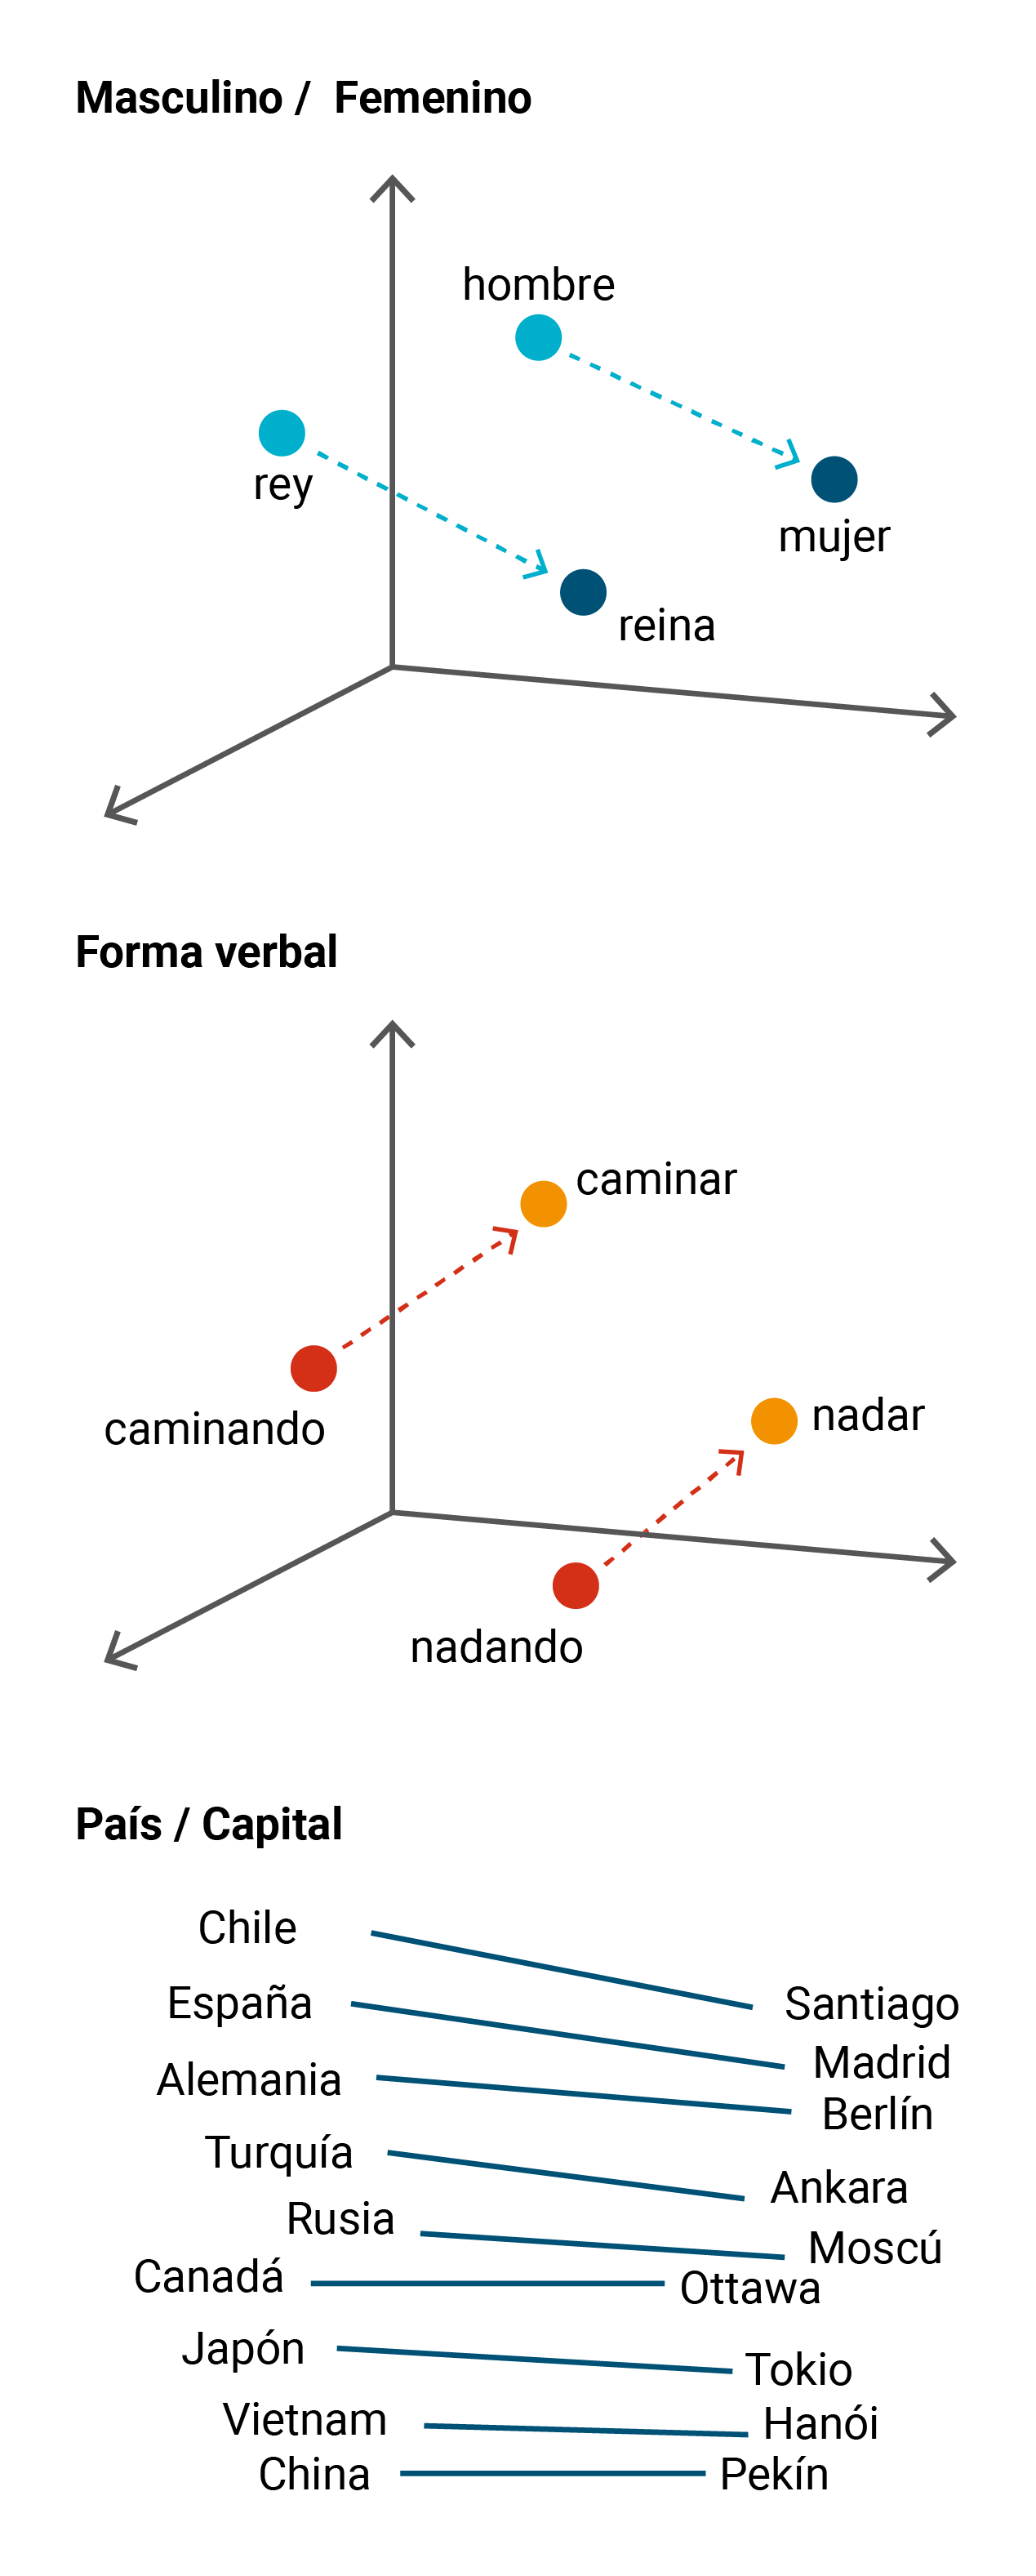
\includegraphics[scale=0.2]{pics/linear-relationships.png}
	\caption{Fuente: \url{https://www.tensorflow.org/tutorials/word2vec}}
\end{figure}

\section{Evaluación}
Existen muchos conjuntos de datos con asociaciones de palabras anotadas por humanos o analogías de oro que se pueden utilizar para evaluar algoritmos de word embeddings.

Estos enfoques se llaman "Enfoques de Evaluación Intrínseca".

La mayoría de ellos están implementados en: \url{https://github.com/kudkudak/word-embeddings-benchmarks}.

Los word embeddings también se pueden evaluar extrínsecamente utilizando en tareas externas de procesamiento del lenguaje natural (por ejemplo, etiquetado de partes del discurso, análisis de sentimientos).

\section{Correspondencia entre modelos distribuidos y distribucionales}
Tanto los métodos distribucionales "basados en recuento" como los distribuidos "neurales" se basan en la hipótesis de distribución.

Ambos intentan capturar la similitud entre palabras basándose en la similitud entre los contextos en los que ocurren.

Levy y Goldebrg mostraron en \cite{levy2014neural} que el modelo Skip-gram con negative sampling (SGNS) está factorizando implícitamente una matriz palabra-contexto, cuyas celdas son la información

mutua puntual (PMI) de los pares respectivos de palabra y contexto, desplazada por una constante global.

Esto vincula los métodos neuronales y los tradicionales "basados en recuento", sugiriendo que en un sentido profundo, las dos familias algorítmicas son equivalentes.

\section{FastText}
Los embeddings de FastText amplían el modelo skipgram teniendo en cuenta la estructura interna de las palabras mientras aprenden las representaciones de las palabras \cite{bojanowski2016enriching}.

Se asocia una representación vectorial con cada $n$-gramo de caracteres.

Las palabras se representan como la suma de estas representaciones.

Tomando la palabra \emph{where} y $n = 3$, se representará por los $n$-gramos de caracteres: $<$wh, whe, her, ere, re$>$, y la secuencia especial $<$where$>$.

Es importante tener en cuenta que la secuencia \emph{$<$her$>$}, correspondiente a la palabra "her", es diferente del tri-grama "her" de la palabra "here".

FastText es útil para los idiomas con una rica morfología. Por ejemplo, las palabras "amazing" y "amazingly" comparten información en FastText a través de sus $n$-gramos compartidos, mientras que en Word2Vec estas dos palabras no tienen ninguna relación.

Sea $\mathcal{G}_{w}$ el conjunto de $n$-gramos que aparecen en $w$.

FastText asocia un vector $\vec{g}$ con cada $n$-gramo en $\mathcal{G}_{w}$.

En FastText, la probabilidad de que un par palabra-contexto $(w, c)$ provenga del corpus de entrada $D$ se calcula de la siguiente manera:

\begin{displaymath}
P(D | w, c) = \frac{1}{1+e^{-s(w,c)}}
\end{displaymath}

donde,

\begin{displaymath}
s(w,c) = \sum_{g \in {G}_{w}} \vec{g} \cdot \vec{c}.
\end{displaymath}

El algoritmo de muestreo negativo se puede calcular de la misma forma que en el modelo skipgram con esta formulación.

\section{Embbedings de frases específicas de sentimiento}
El problema de los embeddings de palabras es que los antónimos pueden usarse en contextos similares, por ejemplo, "mi auto es lindo" vs "mi auto es feo".

En \cite{TangCol14}, se proponen embeddings de palabras específicos de sentimiento combinando el modelo skipgram con tweets con emoticones anotados :) :(.

Estos embeddings se utilizan para entrenar un clasificador de polaridad a nivel de palabra.

El modelo integra la información de sentimiento en la representación continua de frases mediante el desarrollo de una arquitectura neural adaptada.

Entrada: $\{w_i,s_j,pol_j\}$, donde $w_i$ es una frase (o palabra), $s_j$ es la oración y $pol_j$ es la polaridad de la oración.

El objetivo de entrenamiento utiliza el embedding de $w_i$ para predecir las palabras de contexto (de la misma manera que el modelo skipgram) y utiliza la representación de la oración $se_j$ para predecir $pol_j$.

Las oraciones ($se_j$) se representan promediando los vectores de palabras que las componen.

El objetivo de la parte de sentimiento es maximizar el promedio de la probabilidad logarítmica del sentimiento:
\begin{displaymath}
f_{sentimiento}= \frac{1}{S}\sum_{j=1}^{S}\log p(pol_j|se_j)
\end{displaymath}

El objetivo de entrenamiento final es maximizar la combinación lineal de los objetivos skipgram y sentimiento:
\begin{displaymath}
f = \alpha f_{skipgram} + (1- \alpha)f_{sentimiento}
\end{displaymath}

\section{Gensim}
Gensim es una biblioteca de Python de código abierto para el procesamiento del lenguaje natural que implementa muchos algoritmos para entrenar word embeddings.

\begin{itemize}
 \item \url{https://radimrehurek.com/gensim/}
  \item \url{https://machinelearningmastery.com/develop-word-embeddings-python-gensim/}
\end{itemize}

\begin{figure}[h]
	\centering
	
\includegraphics[scale=0.3]{pics/gensim.png}
\end{figure}
